\section{Deep clustering algorithms}\label{sec:convae_clustering}

In the previous section we demonstrated a potential for clustering of events from the AT-TPC experiment. To build on this result we will in this section explore the application of the MIXAE (mixture of autoencoders) algorithm introduced in section \ref{sec:deep_clustering}. The other algorithm introduced in section \ref{sec:deep_clustering}, DCEC (deep clustering with convolutional autoencoders), consistently collapsed to just one cluster for all datasets.

In the MIXAE algorithm the hyper-parameters to adjust are all the ordinary parameters that we introduced in table \ref{tab:convae_hyperparams}. In addition to those parameters come the weighting of the loss terms: $\theta$, $\alpha$ and $\gamma$. These weighting parameters are attached to the reconstruction loss, sample entropy and batch-wise entropy respectively. \cite{Zhang} note that these parameters are very important for the model performance and so we focus primarily on these. 

We empirically freeze the convolutional autoencoder hyperparameters to compress the original $128 \times 128$ to a $8 \times 8$ pixel grid using four convolutional layers. The parameters chosen for the autoencoders are listed in full in table \ref{tab:mixe_ae_hyperparams} 


\begin{table}[H]
\centering
\caption{Hyperparameters selected for the autoencoder components of the MIXAE algorithm, see table \ref{tab:convae_hyperparams} for a full description of the parameters.}\label{tab:mixe_ae_hyperparams}
\setlength{\extrarowheight}{15pt}
\hspace*{-0.5in}
\begin{tabular}{ll}
\toprule
Hyperparameter & Value \\
\midrule
\multicolumn{2}{l}{Convolutional parameters: } \\
\midrule
Number of layers & $4$ \\
Kernels & $[3,\,3,\,3,\,3]$\\
Strides & $[2,\,2,\,2,\,2]$ \\
Filters & $[64,\, 32, \,16, \,8,]$ \\ 
\midrule
\multicolumn{2}{l}{Network parameters: } \\
\midrule
Activation & LRelu \\
Latent type & None \\
Latent dimension & 20  \\
$\beta$ & N/A \\
Batchnorm & False \\
\midrule
\multicolumn{2}{l}{Optimizer parameters: } \\
\midrule
$\eta$ & $10^{-3}$ \\
$\beta_1$ & $0.9$ \\
$\beta_2$ & $0.99$ \\
\bottomrule
\end{tabular}
\end{table}

Since there are then only three remaining hyperparameters we choose to perform a coarse grid-search as described in section \ref{sec:hyperparam_search_arch}.

\begin{table}
\centering
\caption{Hyperparameter grid for the MIXAE loss weighting terms}\label{tab:mixae_loss_weights}
\begin{tabular}{lll}
\toprule
Parameter & Grid & Scale \\
\midrule 
$\theta$ & $[-1,\, 5]$ & Logarithmic \\
$\alpha$ & $[-5,\, -1]$ & Logarithmic \\
$\gamma$ & $[3,\, 5]$ & Logarithmic
\end{tabular}
\end{table}

In contrast with earlier sections we present separate sections for each of the datasets. We begin by considering simulated AT-TPC data

\subsection{Simulated AT-TPC data}

In the clustering algorithm we use the large simulated dataset with $M=80000$ points, evenly distributed between proton- and carbon-events. The algorithm is trained on a subset of $60000$ of these samples, and we track performance on the remaining $20000$ events. 

The grids selected for the search are listed in table \ref{tab:mixae_loss_weights}. The search yielded an optimal configuration with 

\begin{align}
\theta = 10^{-1}, \\
\alpha = 10^{-2}, \\
\gamma = 10^5.
\end{align}

Finally, for these parameters we re-ran the algorithm $N=10$ times to investigate the stability of the algorithm. The results are reported in figure \ref{fig:mixae_sim}. We observe that while the algorithm can achieve very strong performance, i.e. $ARI > 0.8$, it fluctuates strongly. As the batch entropy is consistently low it is not clear how to couple the unsupervised performance with the consistency with the ground truth labels.

\begin{figure}[H]
\centering
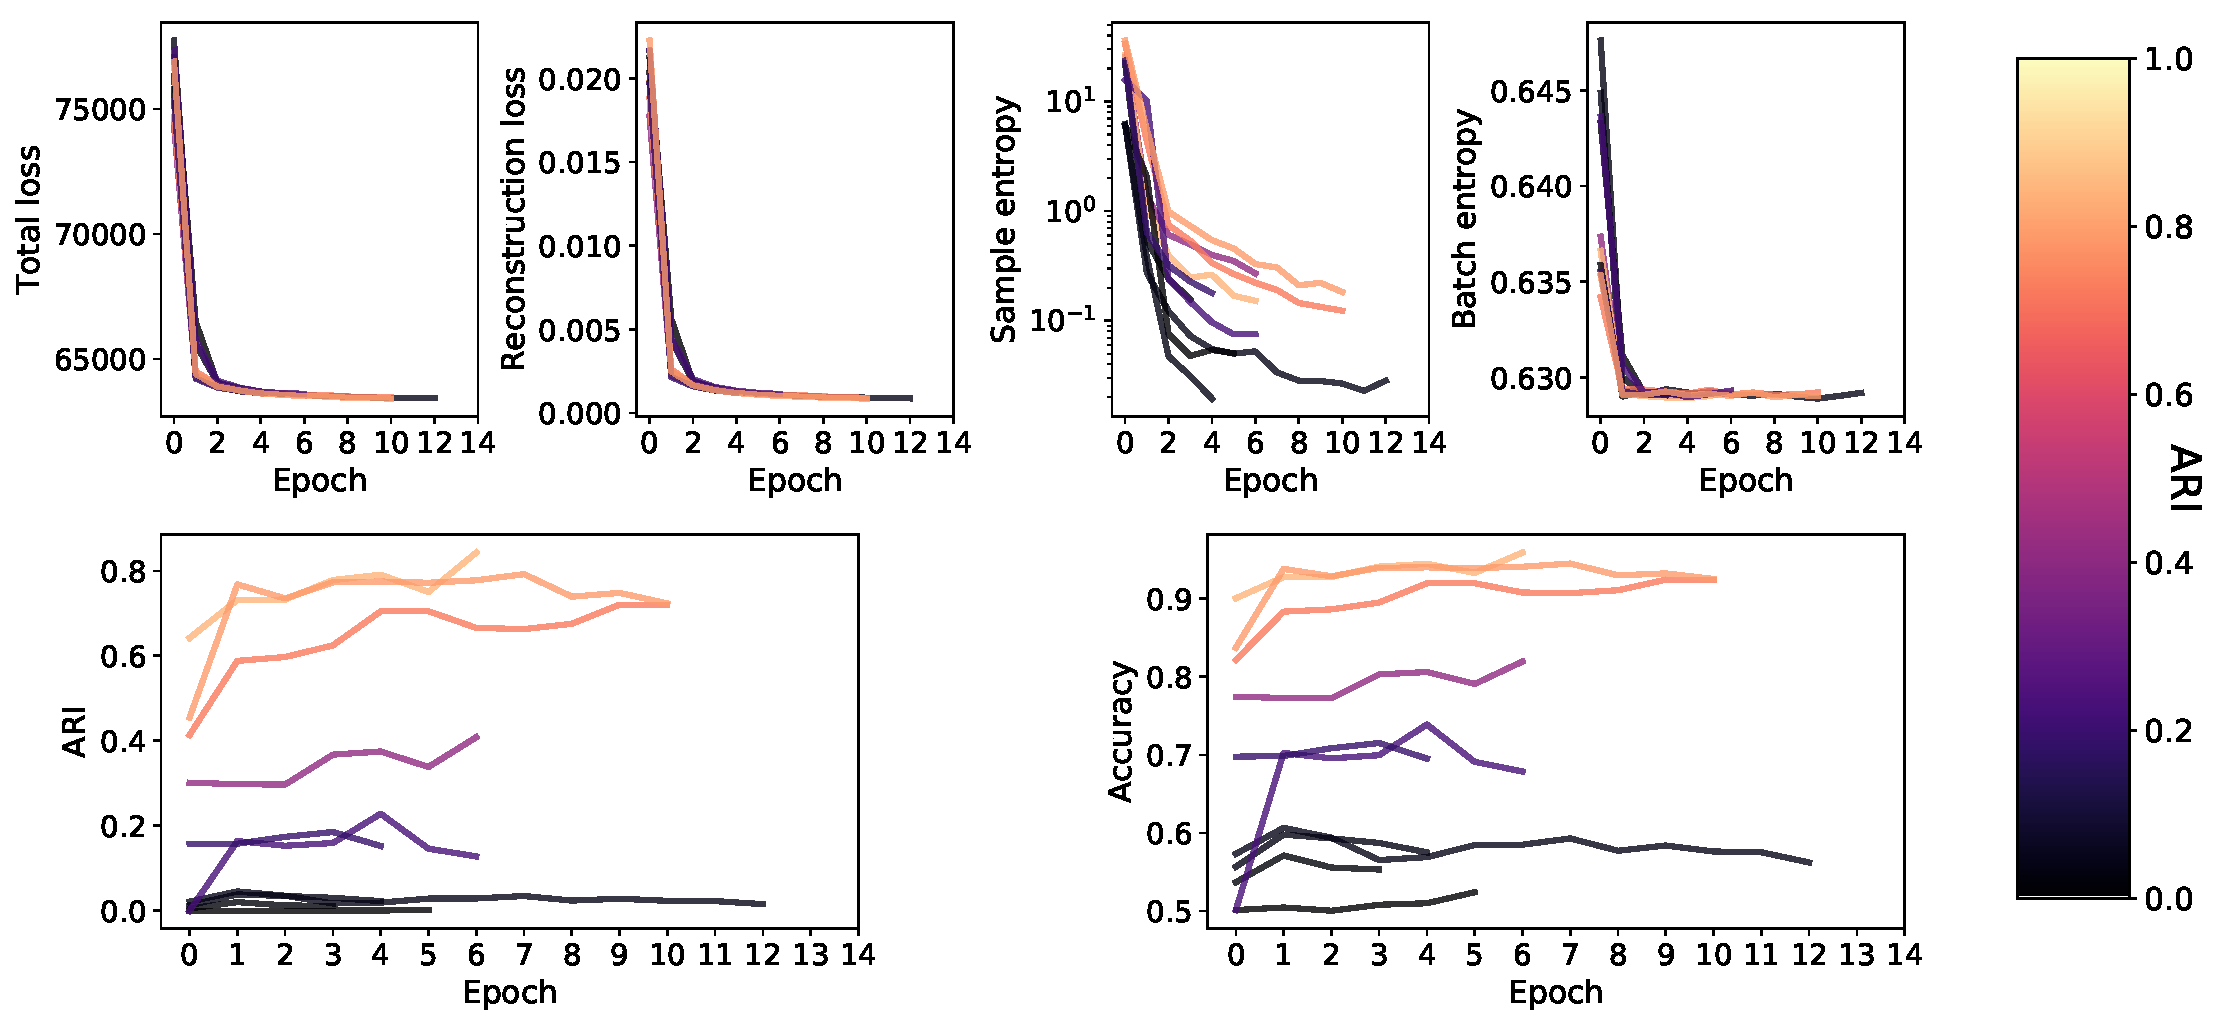
\includegraphics[width=\textwidth]{./plots/sim_mixae.pdf}
\caption{Performance for the MIXAE model on simulated AT-TPC data. In the top row the loss components are plotted for each run, and in the bottom row the ARI (adjusted rand index) and clustering accuracy are shown. Each run is color-coded with the ARI achieved at the end of the run. }\label{fig:mixae_sim}
\end{figure}

\subsection{Filtered AT-TPC data}

We repeat the optimization steps in the previous section for the filtered AT-TPC data. Beginning with a wide grid equal to the grid used for the simulated data we searched over all parameter configurations to find promising values. We then performed a local search around these values to pin-point the hyperparameter configuration. This search yielded the optimal hyper-parameters 

\begin{align}
\theta &= 10^{1}, \\
\alpha &= 10^{-1}, \\
\gamma &= 3.162\times 10^3.
\end{align}

\noindent The results of the runs are included in figure \ref{fig:mixae_clean}. We observe ghat the highest performing models reach an $ARI > 0.5$, which is higher than the performance achieved by the K-means algorithm applied to the VGG16 latent space. 

\begin{figure}[H]
\centering
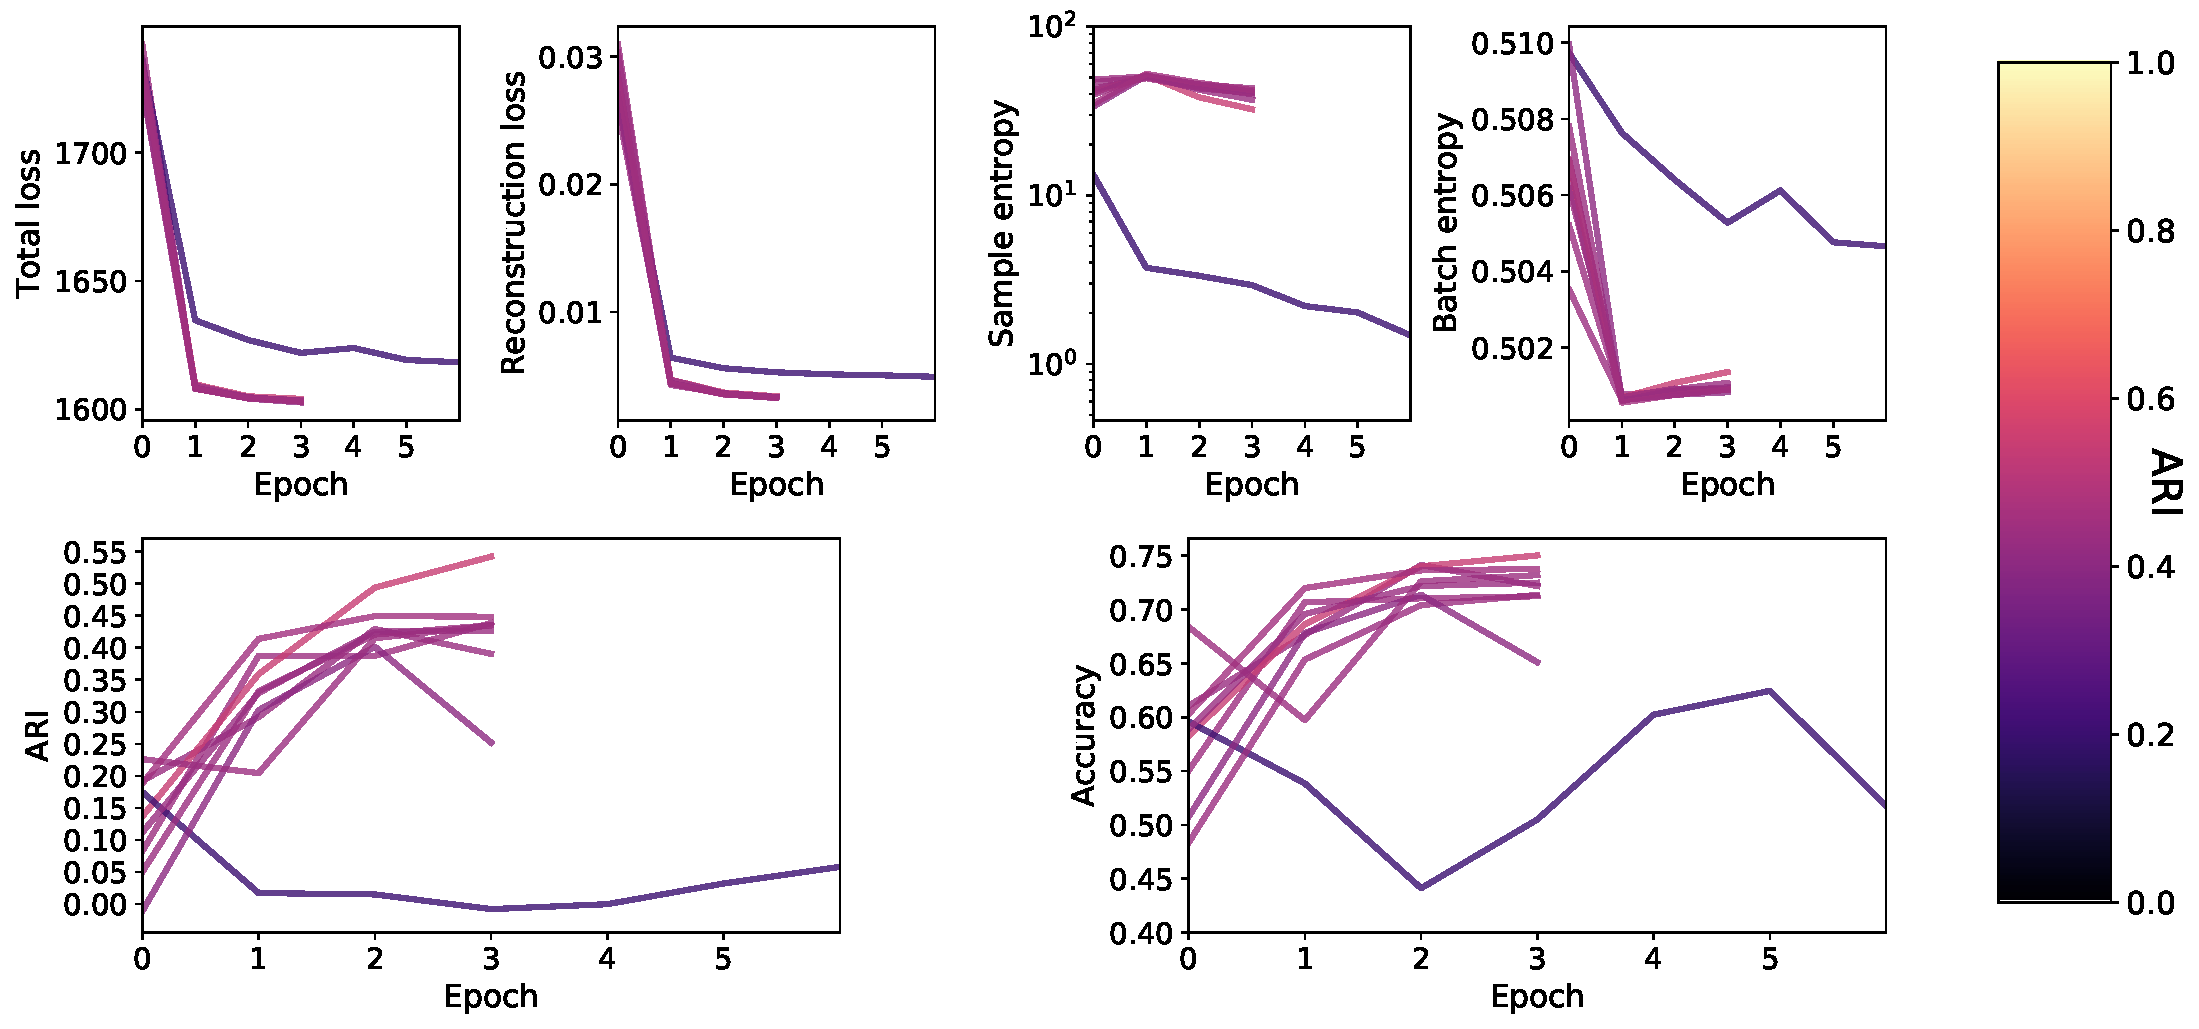
\includegraphics[width=\textwidth]{./plots/clean_mixae.pdf}
\caption{Performance for the MIXAE model on filtered AT-TPC data. In the top row the loss components are plotted for each run, and in the bottom row the ARI (adjusted rand index) and clustering accuracy are shown. Each run is color-coded with the ARI achieved at the end of the run.}\label{fig:mixae_clean}
\end{figure}


\subsection{Full AT-TPC data}

Like the two previous sections we repeat the same procedure of iterative grid searches on the MIXAE loss-weights. Each configuration is re-run a total of $N=10$ times to capture fluctuations in the performance before a final selection is made on the hyperparameters. For the full dataset the MIXAE hyperparameters converge to the same values as for the clean data, i.e. 


\begin{align}
\theta &= 10^{1}, \\
\alpha &= 10^{-1}, \\
\gamma &= 3.162\times 10^3.
\end{align}

\noindent As with the previous datasets we include a plot of the loss curves and performance measures for $N=10$ runs with the same loss-weight parameters, shown in figure \ref{fig:mixae_full}.

\begin{figure}[H]
\centering
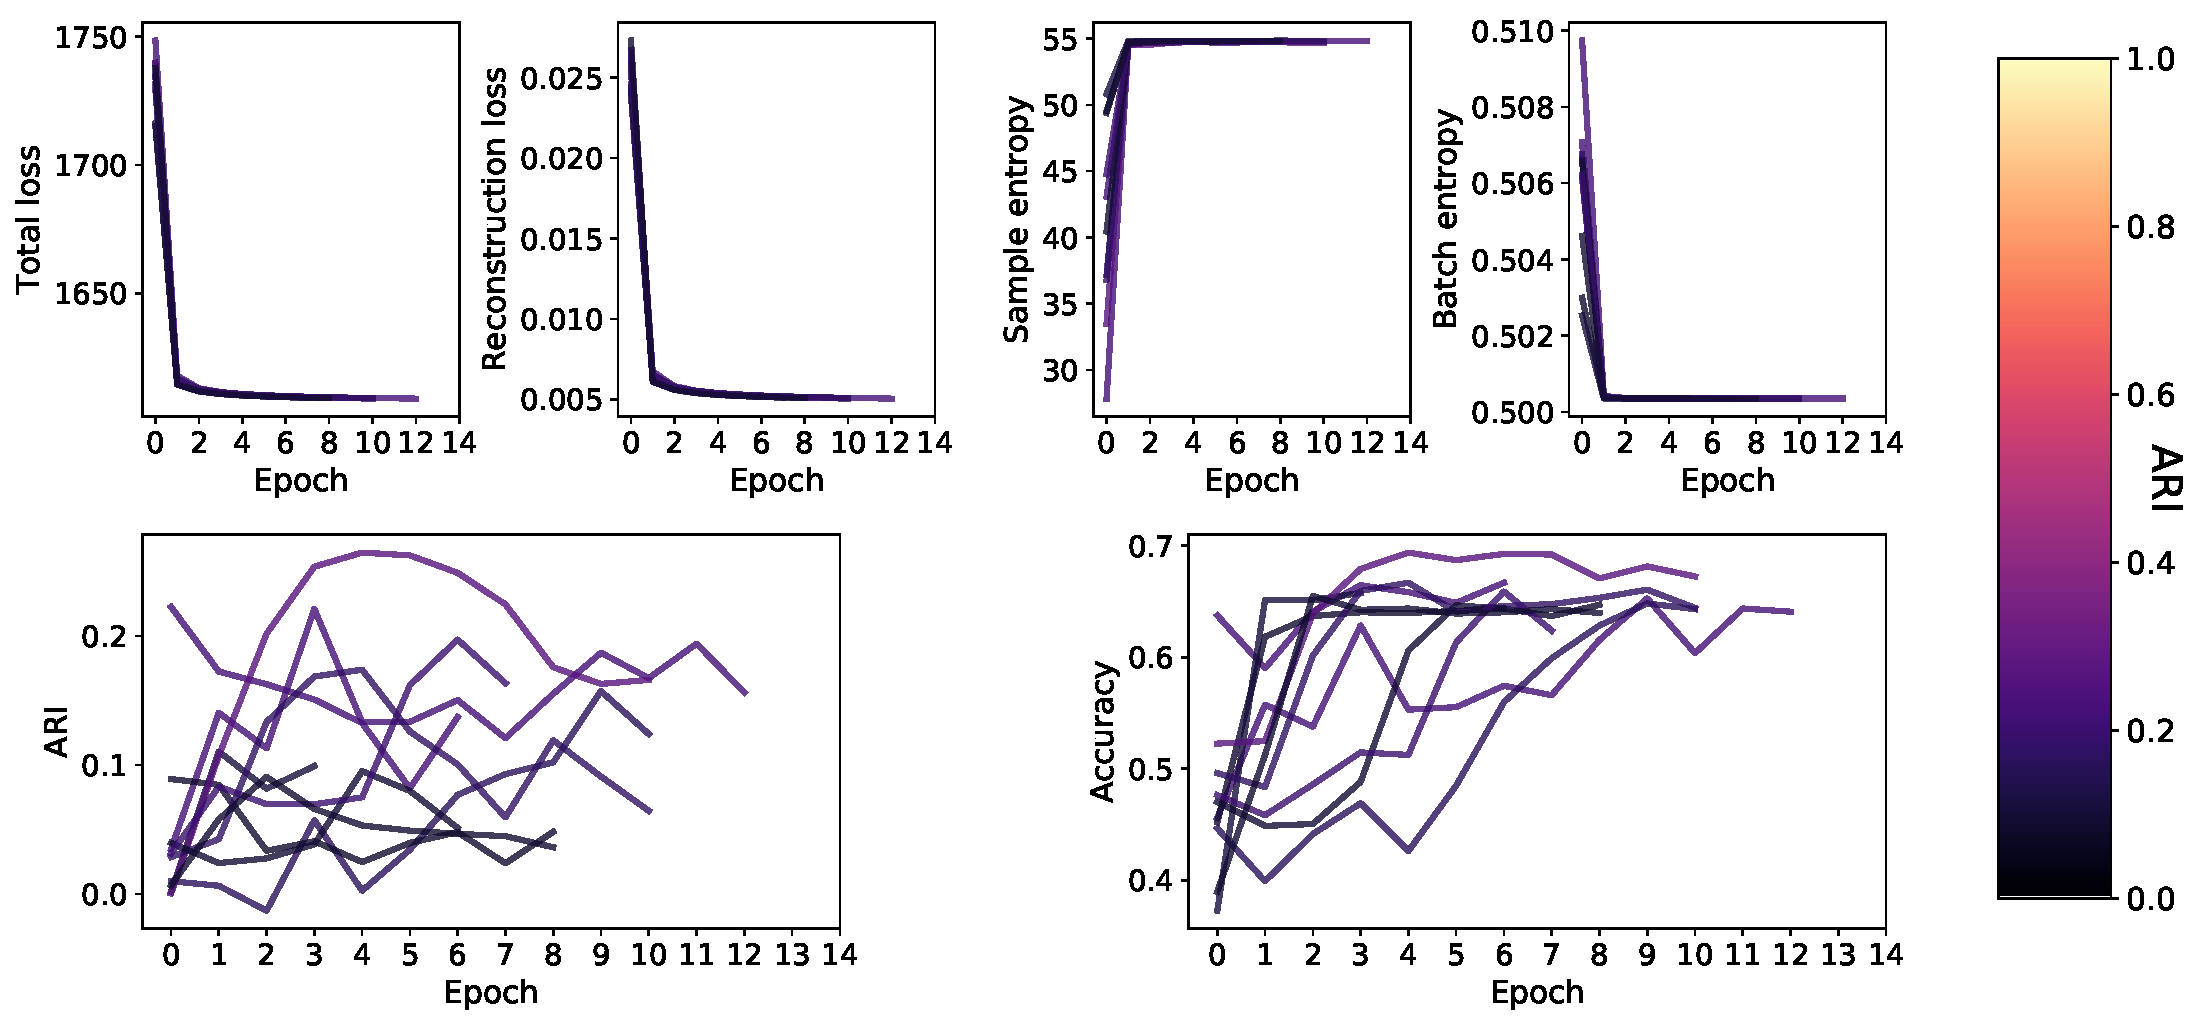
\includegraphics[width=\textwidth]{./plots/real_mixae.pdf}
\caption{Performance for the MIXAE model on un-filtered AT-TPC data. In the top row the loss components are plotted for each run, and in the bottom row the ARI (adjusted rand index) and clustering accuracy are shown. Each run is color-coded with the ARI achieved at the end of the run.}\label{fig:mixae_full}
\end{figure}

\subsection{Comparing performance}

It is also interesting to compare and contrast the clustering results from the MIXAE model with those of the VGG16$+$K-means outside the fairly abstract accuracies and rand scores. It is especially interesting to compare the cluster assignments, as they can inform further research efforts in the clustering of AT-TPC events. The matrices are shown in figure \ref{fig:mixae_confmat}. We observe that the MIXAE applied to the clean data correctly clusters the noise, but incorrectly mixes the proton and carbon classes. Applied to the real data the MIXAE correctly separates the carbon class, however it is unable to separate the proton events from the amorphous noise events.

\begin{figure}[H]
\centering

	\subfloat{
	\includegraphics[width=0.5\textwidth]{plots/filtered_mixae_conf_mat.pdf}
}
	\hspace{-1cm}
	\subfloat{
	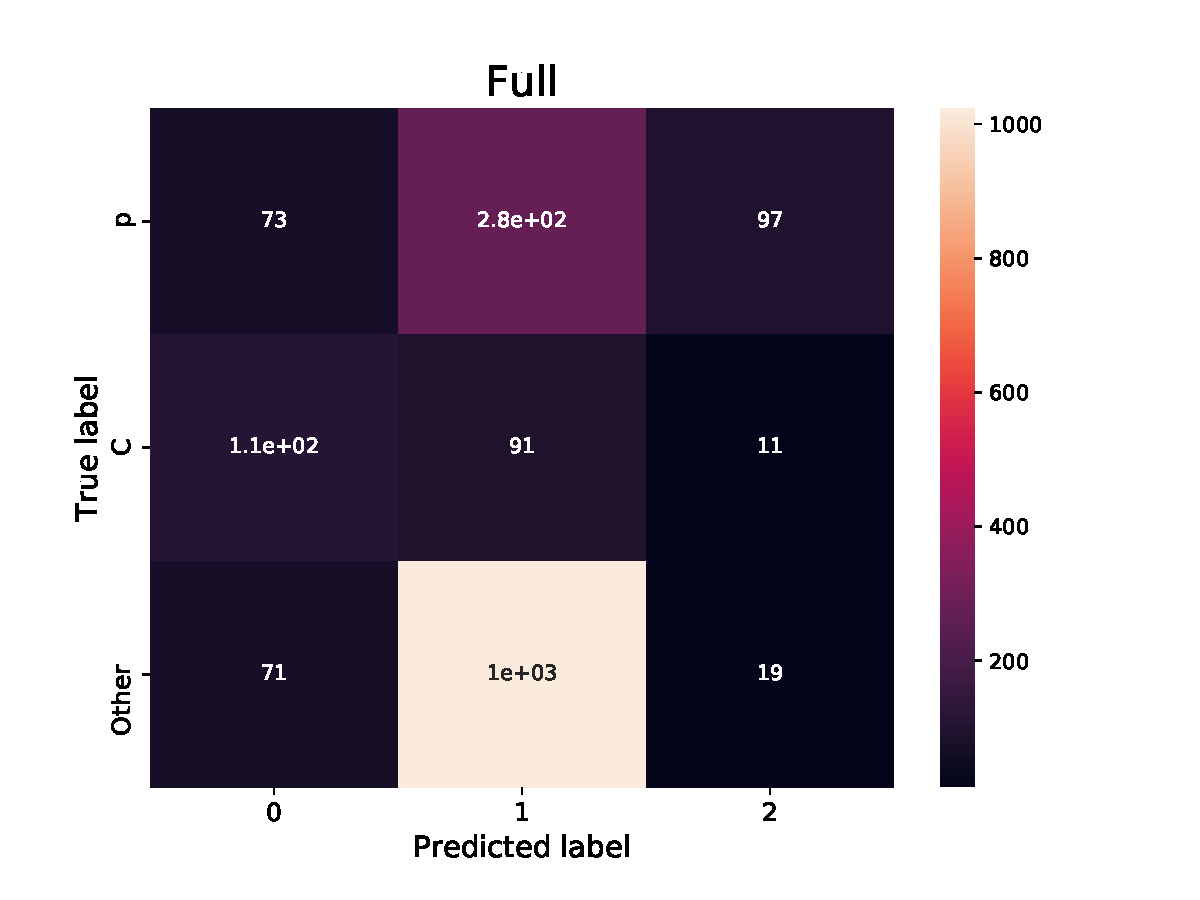
\includegraphics[width=0.5\textwidth]{plots/full_mixae_conf_mat.pdf}
}
\caption[MIXAE - confusion matrices]{Confusion matrices for the MIXAE clustering algorithm on filtered and full AT-TPC events. The true labels indicate samples belonging to the p (proton), C (carbon), or other classes. }\label{fig:mixae_confmat}
\end{figure}